%%%%%%%%%%%%%%%%%%%%%%%%%%%%%%%%%%%%%%%%%
% Beamer Presentation
% LaTeX Template
% Version 1.0 (10/11/12)
%
% This template has been downloaded from:
% http://www.LaTeXTemplates.com
%
% License:
% CC BY-NC-SA 3.0 (http://creativecommons.org/licenses/by-nc-sa/3.0/)
%
%%%%%%%%%%%%%%%%%%%%%%%%%%%%%%%%%%%%%%%%%

%----------------------------------------------------------------------------------------
%	PACKAGES AND THEMES
%----------------------------------------------------------------------------------------

\documentclass[handout]{beamer}

\mode<presentation> {

% The Beamer class comes with a number of default slide themes
% which change the colors and layouts of slides. Below this is a list
% of all the themes, uncomment each in turn to see what they look like.

%\usetheme{default}
%\usetheme{AnnArbor}
%\usetheme{Antibes}
%\usetheme{Bergen}
%\usetheme{Berkeley}
%\usetheme{Berlin}
%\usetheme{Boadilla}
%\usetheme{CambridgeUS}
%\usetheme{Copenhagen}
%\usetheme{Darmstadt}
%\usetheme{Dresden}
%\usetheme{Frankfurt}
%\usetheme{Goettingen}
%\usetheme{Hannover}
%\usetheme{Ilmenau}
%\usetheme{JuanLesPins}
%\usetheme{Luebeck}
\usetheme{Madrid}
%\usetheme{Malmoe}
%\usetheme{Marburg}
%\usetheme{Montpellier}
%\usetheme{PaloAlto}
%\usetheme{Pittsburgh}
%\usetheme{Rochester}
%\usetheme{Singapore}
%\usetheme{Szeged}
%\usetheme{Warsaw}

% As well as themes, the Beamer class has a number of color themes
% for any slide theme. Uncomment each of these in turn to see how it
% changes the colors of your current slide theme.

%\usecolortheme{albatross}
%\usecolortheme{beaver}
%\usecolortheme{beetle}
%\usecolortheme{crane}
%\usecolortheme{dolphin}
%\usecolortheme{dove}
%\usecolortheme{fly}
%\usecolortheme{lily}
%\usecolortheme{orchid}
%\usecolortheme{rose}
%\usecolortheme{seagull}
%\usecolortheme{seahorse}
%\usecolortheme{whale}
%\usecolortheme{wolverine}

%\setbeamertemplate{footline} % To remove the footer line in all slides uncomment this line
%\setbeamertemplate{footline}[page number] % To replace the footer line in all slides with a simple slide count uncomment this line

%\setbeamertemplate{navigation symbols}{} % To remove the navigation symbols from the bottom of all slides uncomment this line
}

\usepackage{graphicx} % Allows including images
\usepackage{booktabs} % Allows the use of \toprule, \midrule and \bottomrule in tables
\usepackage{cool}
\usepackage{tikz}
\usepackage{amsmath}
\usepackage{xcolor}
\usepackage{hyperref}
\usepackage{bm}

\DeclareMathOperator*{\argmax}{argmax}
\DeclareMathOperator*{\argmin}{argmin}
\usetikzlibrary{positioning}

%----------------------------------------------------------------------------------------
%	TITLE PAGE
%----------------------------------------------------------------------------------------

\title[ML for Retail]{Forecasting and Decisioning in Retail} % The short title appears at the bottom of every slide, the full title is only on the title page

\author{Ashwin Rao} % Your name
\institute[Stanford] % Your institution as it will appear on the bottom of every slide, may be shorthand to save space
{Stanford University
 % Your institution for the title page
}

\date{} % Date, can be changed to a custom date

\begin{document}
\begin{frame}
\titlepage % Print the title page as the first slide
\end{frame}

% \begin{frame}
% \frametitle{Overview} % Table of contents slide, comment this block out to remove it
% \tableofcontents % Throughout your presentation, if you choose to use \section{} and \subsection{} commands, these will automatically be printed on this slide as an overview of your presentation
% \end{frame}


\begin{frame}
\frametitle{A bit about me}
\pause
\begin{itemize}[<+->]
\item Co-Founder of CX Score: AI to improve Customer Experience on Apps
\item Adjunct Professor, \href{https://icme.stanford.edu/}{\underline{\textcolor{blue}{Applied Mathematics (ICME)}}}, Stanford University
\item Past: VP of AI at Target Corporation
\item Past: MD at Morgan Stanley, Trading Strategist at Goldman Sachs
\item I direct Stanford's \href{https://mcf.stanford.edu/}{\underline{\textcolor{blue}{Mathematical \& Computational Finance program}}}
\item Research \& Teaching in: {\em RL and it's applications in Finance \& Retail}
\item Book:  \href{https://www.amazon.com/Foundations-Reinforcement-Learning-Applications-Finance/dp/1032124121}{\underline{\textcolor{blue}{Foundations of RL with Applications in Finance}}}
\item CX Score uses RL as it's core technology
\item Lived in Mumbai, LA, NYC, London, now settled in Palo Alto
\item Today I will talk about Forecasting and Decisioning in Retail
\end{itemize}
\end{frame}

\section{Machine Learning Overview}

\begin{frame}
\frametitle{Machine Learning Branches}
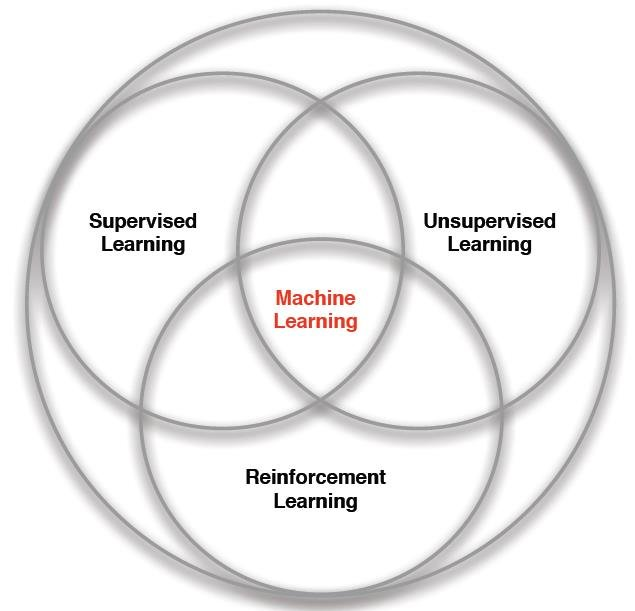
\includegraphics[width=9cm, height=8cm]{../finance/cme241/MLBranches.PNG}
\end{frame}

\begin{frame}
\frametitle{Machine Learning Overview}
\pause
\begin{itemize}[<+->]
\item ML is roughly classified into Supervised, Unsupervised and RL
\item Supervised: Predicts by learning relationships between variables
\item Unsupervised: Unearths patterns \& structures within data
\item RL: Optimal Sequential Decisioning under Uncertainty
\item ML has been a breakthrough for images, text, games
\item Largely due to the past decade of success of Deep Neural Networks
\item We are now adapting Deep Learning techniques to other domains
\item Works well when we have plenty of data and plenty of compute
\item ML practice tends to be quite laborious on Big Data Engineering
\item I've seen promising results in Finance and Retail applications
\item I cover this in depth in my \href{https://www.amazon.com/Foundations-Reinforcement-Learning-Applications-Finance/dp/1032124121}{\underline{\textcolor{blue}{book}}}
\end{itemize}
\end{frame}


\section{Supply-Chain}

\begin{frame}
\frametitle{Supply-Chain Headaches and Machine Learning Pills}
\pause
\begin{itemize}[<+->]
\item Customer Demand is hard to forecast
\item We've had significant supply challenges since Covid started
\item Often, Space and Throughput constraints
\item Network Planning, Labor Planning, Transportation - all challenging
\item Tracking Inventory Count/Location is hard
\item Not easy to control damage, theft, misplacement, spoilage
\item Nirvana: Inventory at right time/place, in right quantity, at low cost
\item Blend of Traditional OR + Modern ML paves the path to Nirvana
\item Today we look at two game-changing applications of ML
\item Demand Forecasting and Inventory Replenishment
\end{itemize}
\end{frame}

\section{Demand Forecasting: Transformers and Embeddings to the rescue}

\begin{frame}
\frametitle{Demand Forecasting}
\pause
\begin{itemize}[<+->]
\item Why do we care about Demand Forecasting?
\item Because it is foundational to LOTs of decisions in Supply-Chain
\item Design/Planning Decisions and Operational/Control Decisions
\item Design/Planning examples: Network, Labor, Transportation
\item Operational/Control examples: Replenishment, Logistics
\item Core: Forecast demand for [SKU group, locations group, time range]
\item Identify your problem's slice thickness in each of these 3 dimensions
\item Thin Slice (local effects): Little data, highly uncertain forecasts
\item Thick Slice (macro effects): Dependent on many external factors
\item Hierarchical forecasting blends macro effects with local effects
\item Good forecast captures structural patterns along with regime shifts
\end{itemize}
\end{frame}

\begin{frame}
\frametitle{Similar/Substitutable Products identified with {\em Embeddings}}
\pause
\begin{itemize}[<+->]
\item Demand Forecasting for similar/substitutable set of Products
\item Can we automate identification of similarity/substitutability?
\item Similarity by Visuals or by Descriptions or by Customer Interest
\item Throw this heterogeneous data into deep neural network learning
\item Deep inside the neural network, we find encodings of these products
\item Similar/Substitutable products have similar encodings
\item The technical term for these encodings is \href{https://developers.google.com/machine-learning/crash-course/embeddings/video-lecture}{\underline{\textcolor{blue}{Embeddings}}}
\item Embeddings are low-dimensional numerical representations ({\em Vectors})
\item Capturing the most important features of products
\item Captures various relationships between products, eg: complementarity
\item Based on product images, descriptions, customer interest
\item Embeddings can be used as ML features for transfer learning
\item Embedding vectors have powerful algebraic/geometric properties
\end{itemize}
\end{frame}

\begin{frame}
\frametitle{Book Embeddings flattened to 2-D Vectors}
\includegraphics[width=12cm, height=8cm]{../supply_chain/BookEmbeddings.png}
\end{frame}

\begin{frame}
\frametitle{Transformers for learning the old and the new}
\pause
\begin{itemize}[<+->]
\item Forecasting needs to be ``Predictive'' as well as ``Reactive''
\item {\em Predictive:} Capture temporal patterns from long history
\item {\em Reactive:} Pay attention to recent shifts and trends
\item \href{https://en.wikipedia.org/wiki/Transformer_(machine_learning_model)}{\underline{\textcolor{blue}{Transformer Networks}}} eating the lunch of good old time-series stats
\item The core methodology is a technique called {\em Self-Attention}
\item It automatically identifies the relative importance of old versus new
\item Transformers are accurate and fast (highly parallelizable)
\item Have found great success in Vision and Text applications
\item Now being ported to numerical time-series applications
\item Embeddings blended with Transformers $\Rightarrow$ Practically Potent Combo
\item Not easy to pull off, requires considerable experimentation/tuning
\end{itemize}
\end{frame}

\begin{frame}
\frametitle{Capturing Stock Price Cycles/Trends with Transformers}
\includegraphics[width=11cm, height=7cm]{../supply_chain/StockPriceTransformer.jpeg}
\end{frame}

\section{Inventory Replenishment: Reinforcement Learning to the rescue}


\begin{frame}
\frametitle{Inventory Replenishment}
\pause
\begin{itemize}[<+->]
\item Let's consider a simple example of a single SKU in a store
\item The store experiences uncertain daily customer demand
\item The store can order daily from a supplier carrying infinite inventory
\item Cost associated with ordering, and order arrives in a few days
\item Inventory in the store incurs a daily {\em Holding Cost} (per unit)
\item Out-of-Stock incurs a {\em Stockout Cost} (per unit)
\item There's a notion of {\em Ordering Cost} (Labor/Transport)
\item When should one order? And in what quantity?
\item Traditional OR literature focused on closed-form ``solutions''
\item Approx closed-form solutions are often used in real businesses
\item In spite of the limitations of missing out on key real-world features
\end{itemize}
\end{frame}


\begin{frame}
\frametitle{Welcome to the Real-World}
\pause
\begin{itemize}[<+->]
\item Real-world not so simple - frictions, constraints, uncertainties
\item Supply can be constrained/uncertain
\item Space and Throughput constraints
\item Pricing/Marketing has a big influence on demand
\item New products, substitutable products complicate matters
\item In physical stores, there are {\em Presentation-Minimum} requirements
\item Often, products are shipped in casepacks
\item Irregular/Uncertain order frequency and lead times
\item Supply-Chain network might be {\em Multi-Echelon}
\item Inventory Count/Location is often uncertain
\item Cost of Damage, Theft, Misplacement, Spoilage
\item End-of-Season/Obsolescence/Spoilage requires Clearance/Salvage
\item All of this calls for a formal Decision Control framework
\end{itemize}
\end{frame}



\begin{frame}
\frametitle{The \href{https://en.wikipedia.org/wiki/Markov_decision_process}{\underline{\textcolor{yellow}{Markov Decision Process}}} Framework}
\includegraphics[width=12cm, height=7cm]{../finance/cme241/MDP.png}
\end{frame}

\begin{frame}
\frametitle{Components of the MDP Framework}
\pause
\begin{itemize}[<+->]
\item The {\em Agent} and the {\em Environment} interact in a time-sequenced loop
\item {\em Agent} responds to [{\em State}, {\em Reward}] by taking an {\em Action}
\item {\em Environment} responds by producing next step's (random) {\em State}
\item {\em Environment} also produces a (random) number we call {\em Reward}
\item Goal of {\em Agent} is to maximize {\em Expected Sum} of all future {\em Reward}s
\item By controlling the ({\em Policy} : {\em State} $\rightarrow$ {\em Action}) function
\item This is a dynamic (time-sequenced control) system under uncertainty
\item MDP framework enables modeling real-world Replenishment problems
\end{itemize}
\end{frame}

\begin{frame}
\frametitle{How a baby learns to walk}
\includegraphics[width=13cm, height=8cm]{../finance/cme241/BabyMDP.jpg}
\end{frame}

\begin{frame}
\frametitle{Many real-world problems fit this MDP framework}
\pause
\begin{itemize}[<+->]
\item Self-driving vehicle (speed/steering to optimize safety/time)
\item Game of Chess (Boolean {\em Reward} at end of game)
\item Inventory Replenishment to ensure high availability at low cost
\item Make a humanoid robot walk/run on difficult terrains
\item Manage an investment portfolio (covered in depth in my book)
\item Control a power station
\item Optimal decisions during a football game
\item Strategy to win an election (high-complexity MDP)
\end{itemize}
\end{frame}

\begin{frame}
\frametitle{Self-Driving Vehicle}
\includegraphics[width=13cm, height=8cm]{../finance/cme241/CarMDP.jpg}
\end{frame}

\begin{frame}
\frametitle{Real-World Replenishment as a Markov Decision Process}
\pause
\begin{itemize}[<+->]
\item MDP {\em State} is current Inventory Level at the store/warehouse
\item {\em State} also includes current in-transit inventory
\item {\em Action} is the multiple of casepack to order (or not order)
\item {\em Reward} function involves all of the costs we went over
\item State transitions governed by all of the uncertainties we went over
\item Solve: \href{https://en.wikipedia.org/wiki/Dynamic_programming}{\underline{\textcolor{blue}{Dynamic Programming}}} or
 \href{https://en.wikipedia.org/wiki/Reinforcement_learning}{\underline{\textcolor{blue}{Reinforcement Learning}}}
\item Curse of Dimensionality and Curse of Modeling $\Rightarrow$ RL
\end{itemize}
\end{frame}


\begin{frame}
\frametitle{How RL Works: Learning from Samples of Data}
\pause
\begin{itemize}[<+->]
\item RL incrementally learns from state/reward transitions data
\item Typically served by a simulator acting as a {\em Simulated Environment}
\item RL is a ``trial-and-error'' approach linking {\em Actions} to {\em Rewards}
\item Try different actions \& learn what works, what doesn't
\item Deep Neural Networks are typically used for function approximation
\item Big Picture: Sampling and Function Approximation come together
\item RL algorithms are clever about balancing  ``explore'' versus ``exploit''
\item Promise of modern A.I. is based on success of RL algorithms
\item Potential for automated decision-making in many industries
\item In 10-20 years: Bots that act or behave more optimal than humans
\item RL already solves various low-complexity real-world problems
\item RL has many applications in Suppy-Chain, more broadly in Operations
\item RL covered in great detail in my book (theory, code and applications)
\end{itemize}
\end{frame}

\section{Clearance Price Optimization}

\begin{frame}
\frametitle{Clearance Price Optimization}
\pause
\begin{itemize}[<+->]
\item You are a few weeks away from end-of-season (eg: Christmas Trees)
\item Assume you have too much inventory in your store
\item What is the optimal sequence of price markdowns?
\item Under (uncertain) demand responding to markdowns
\item So as to maximize your total profit (sales revenue minus costs)
\item Note: There is a non-trivial cost of performing a markdown
\item If price markdowns are small, we end up with surplus at season-end
\item Surplus often needs to be disposed at poor salvage price
\item If price reductions are large, we run out of Christmas trees early
\item ``Stockout'' cost is considered to be large during holiday season
\item This can be modeled as a Markov Decision Process
\end{itemize}
\end{frame}

\begin{frame}
\frametitle{MDP for Clearance Price Optimization}
\pause
\begin{itemize}[<+->]
\item {\em State} is [Days Left, Current Inventory, Current Price, Market Info]
\item {\em Action} is Price Markdown
\item {\em Reward} includes Sales revenue, markdown cost, stockout cost, salvage
\item {\em Reward} \& {\em State}-transitions governed by {\em Price Elasticity of Demand}
\item Real-world {\em Model} can be quite complex (eg: competitor pricing)
\item Big Idea: Blend Inventory and Price Optimization into one MDP
\end{itemize}
\end{frame}

\begin{frame}
\frametitle{Components of Clearance Pricing A.I.}
\pause
\begin{itemize}[<+->]
\item Statistical Estimation of {\em Price Elasticity of Demand}
\item Backward Induction algorithm for Optimal Dynamic Pricing
\item Simulation of the Optimal Policy to reveal various metrics to analyze
\end{itemize}
\end{frame}

\begin{frame}
\frametitle{Optimal Pricing as a function of Inventory and Time}
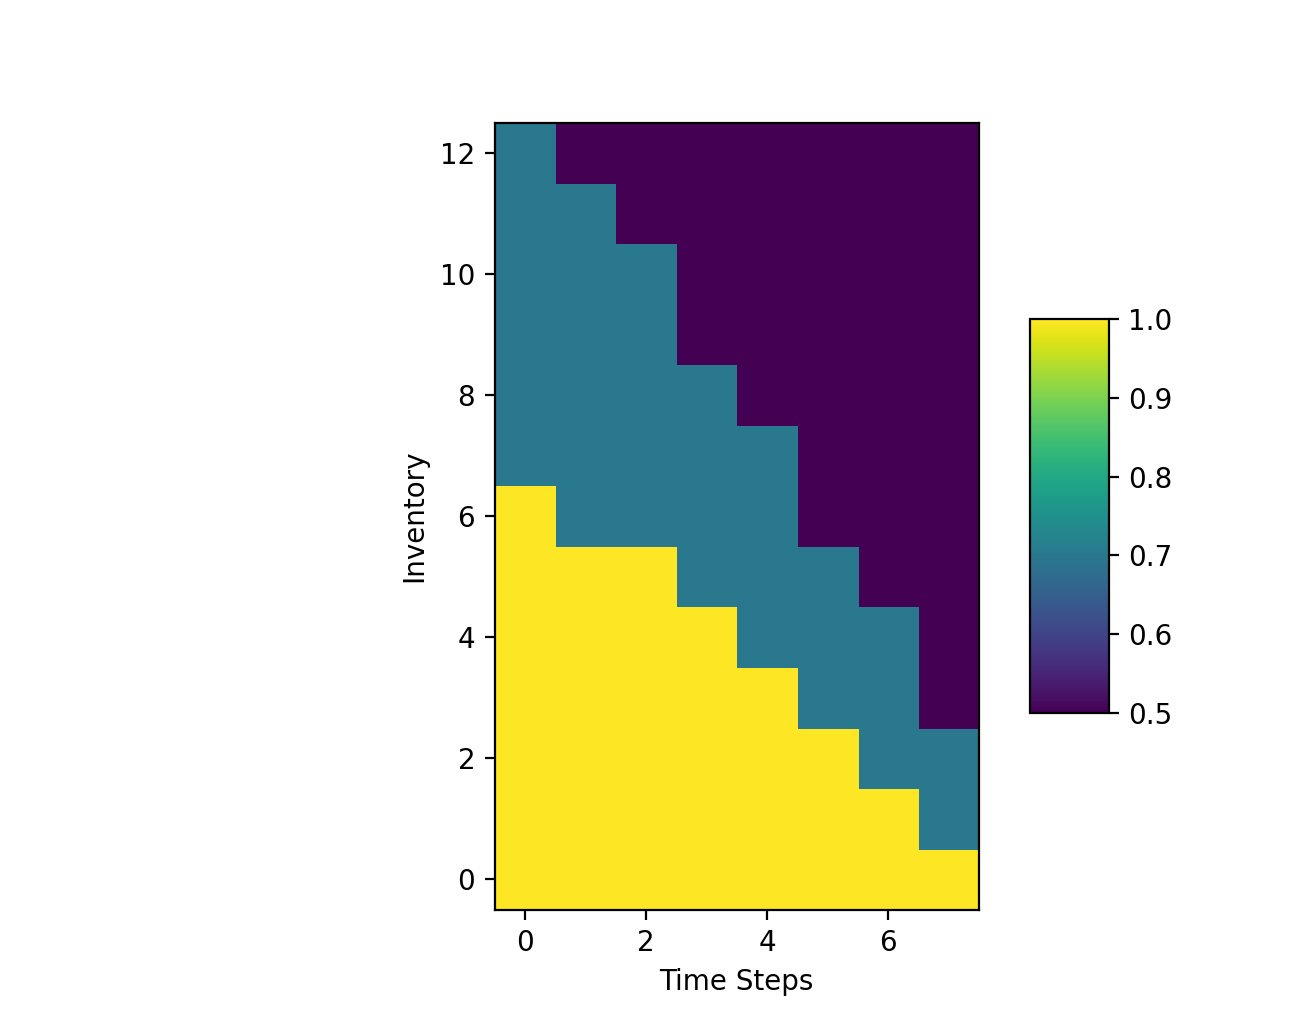
\includegraphics[width=12cm, height=8cm]{dynamic_pricing.png}
\end{frame}


\end{document}